\section{Autopilot for course hold using aileron and successive loop closure}
\subsection{}
The transfer function relates $\delta_a$ and $p$ through an integrator. Therefore, we extract $\dot{p}$ from the state-space vector. 
\begin{align*}
    \dot{p} &= -10.6 \beta - 2.87 p + 0.46 r - 0.65 \delta_a \\
    (s + 2.87) p &= - 0.65 \delta_a  + \frac{(-10.6 \beta + 0.46 r) \delta_a }{\delta_a} \\
    \frac{p}{\delta_a} &= \frac{-0.65}{s + 2.87} + \frac{-10.6 \beta + 0.46 r}{(s + 2.87)\delta_a}
\end{align*}

Then, as this controller is concerned with the roll, we may assume: % that $\beta \approx 0$ and $\r \approx 0$. Therefore, we can conclude that $a_{\phi_1} = 2.87$ and $a_{\phi_2} = -0.65$
\begin{align*}
    \beta \approx 0 && r \approx 0
\end{align*}
And may conclude: 
\begin{align*}
    a_{\phi_1} = 2.87 && a_{\phi_2} = -0.65
\end{align*}

\subsection{}
Using equations 6.7, 6.8 and 6.9 from \cite[page 100]{beard_mclain_2012}, we get: 

\begin{align*}
    k_{p_\phi} &= \frac{\delta_{a}^{\max}}{e_{\phi}^{\max}} sign(a_{\phi_2}) 
    = - \frac{30 \degree}{15 \degree} sign(-0.65)
    = -2 \\
    \omega_{n_{\phi}} &= \sqrt{|a_{\phi_2}| \frac{\delta_a^{\max}}{e_{\phi}^{\max}}} 
    = \sqrt{0.65 * \frac{30 \degree}{15 \degree}} 
    \approx 1.140 \\
    k_{d_\phi} &= \frac{2 \zeta_{\phi} \omega_{n_\phi} - a_{\phi_1}}{a_{\phi_2}} 
    = \frac{2 * 0.707 * 1.140 - 2.87}{-0.65}
    \approx 1.935
\end{align*}

Then using the Evans form from \cite[page 102]{beard_mclain_2012} and the $rlocus$ function from Matlab, we get: 

\subsection{}
\begin{figure}[ht]
	\centering
	\begin{subfigure}[b]{0.45\textwidth}
		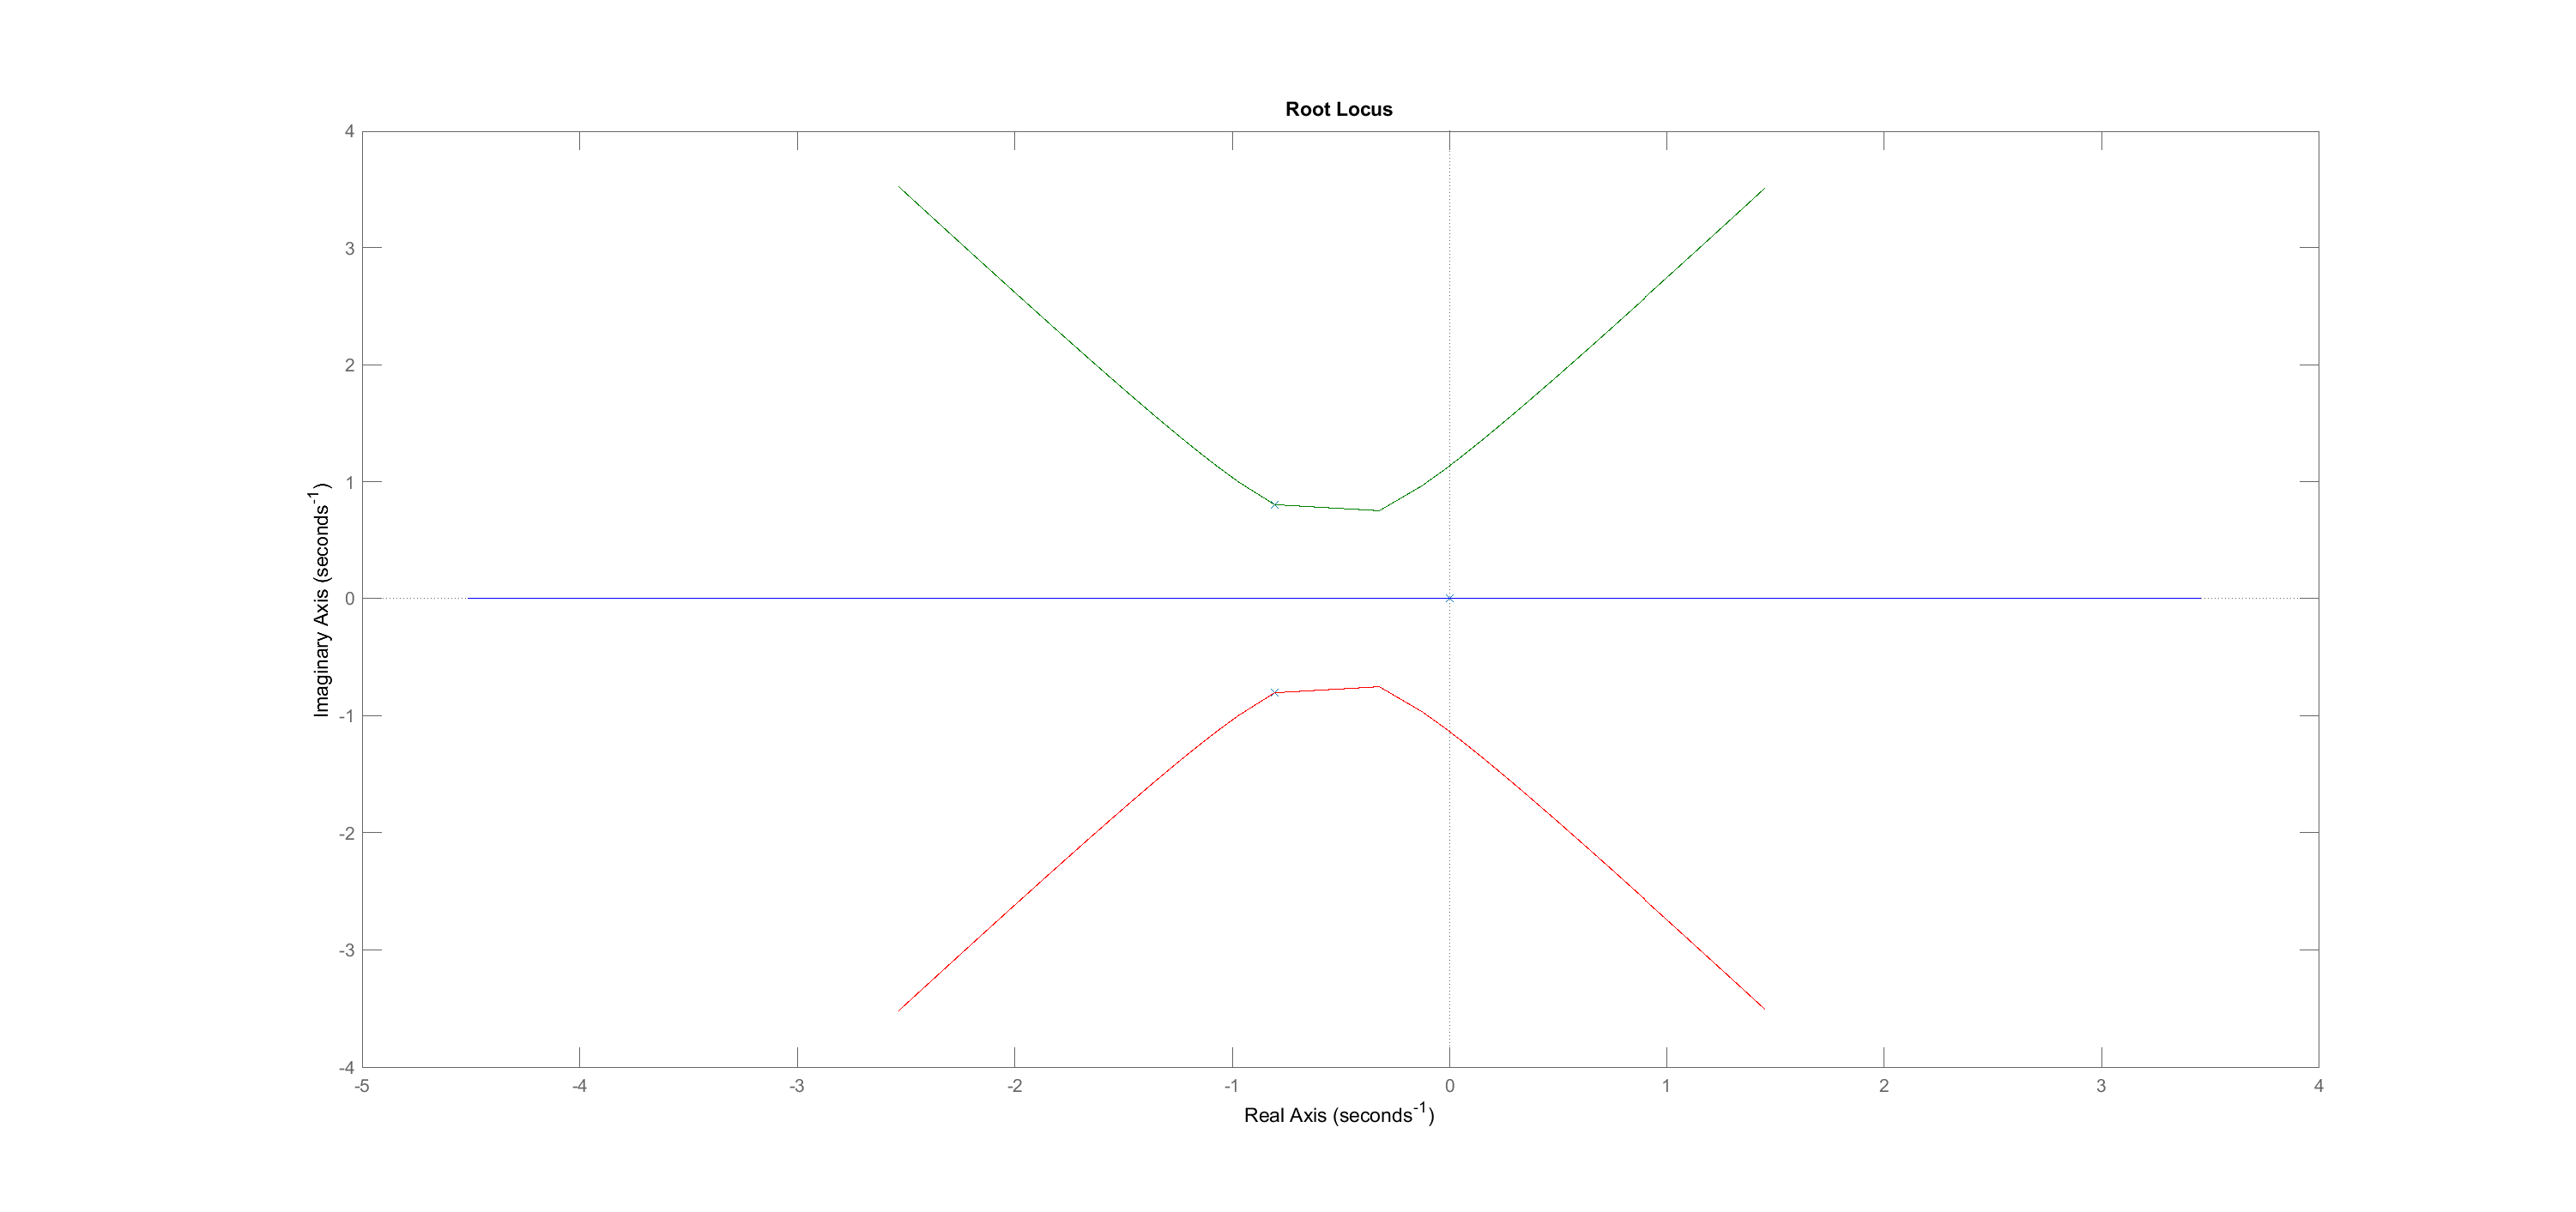
\includegraphics[width=\textwidth]{figures/root_locus_k_i_phi}
		\caption{Root locus with range $k_{i_\phi}$ from -100 to 100}
		\label{fig:root_locus_large_range}
	\end{subfigure}
	\begin{subfigure}[b]{0.45\textwidth}
		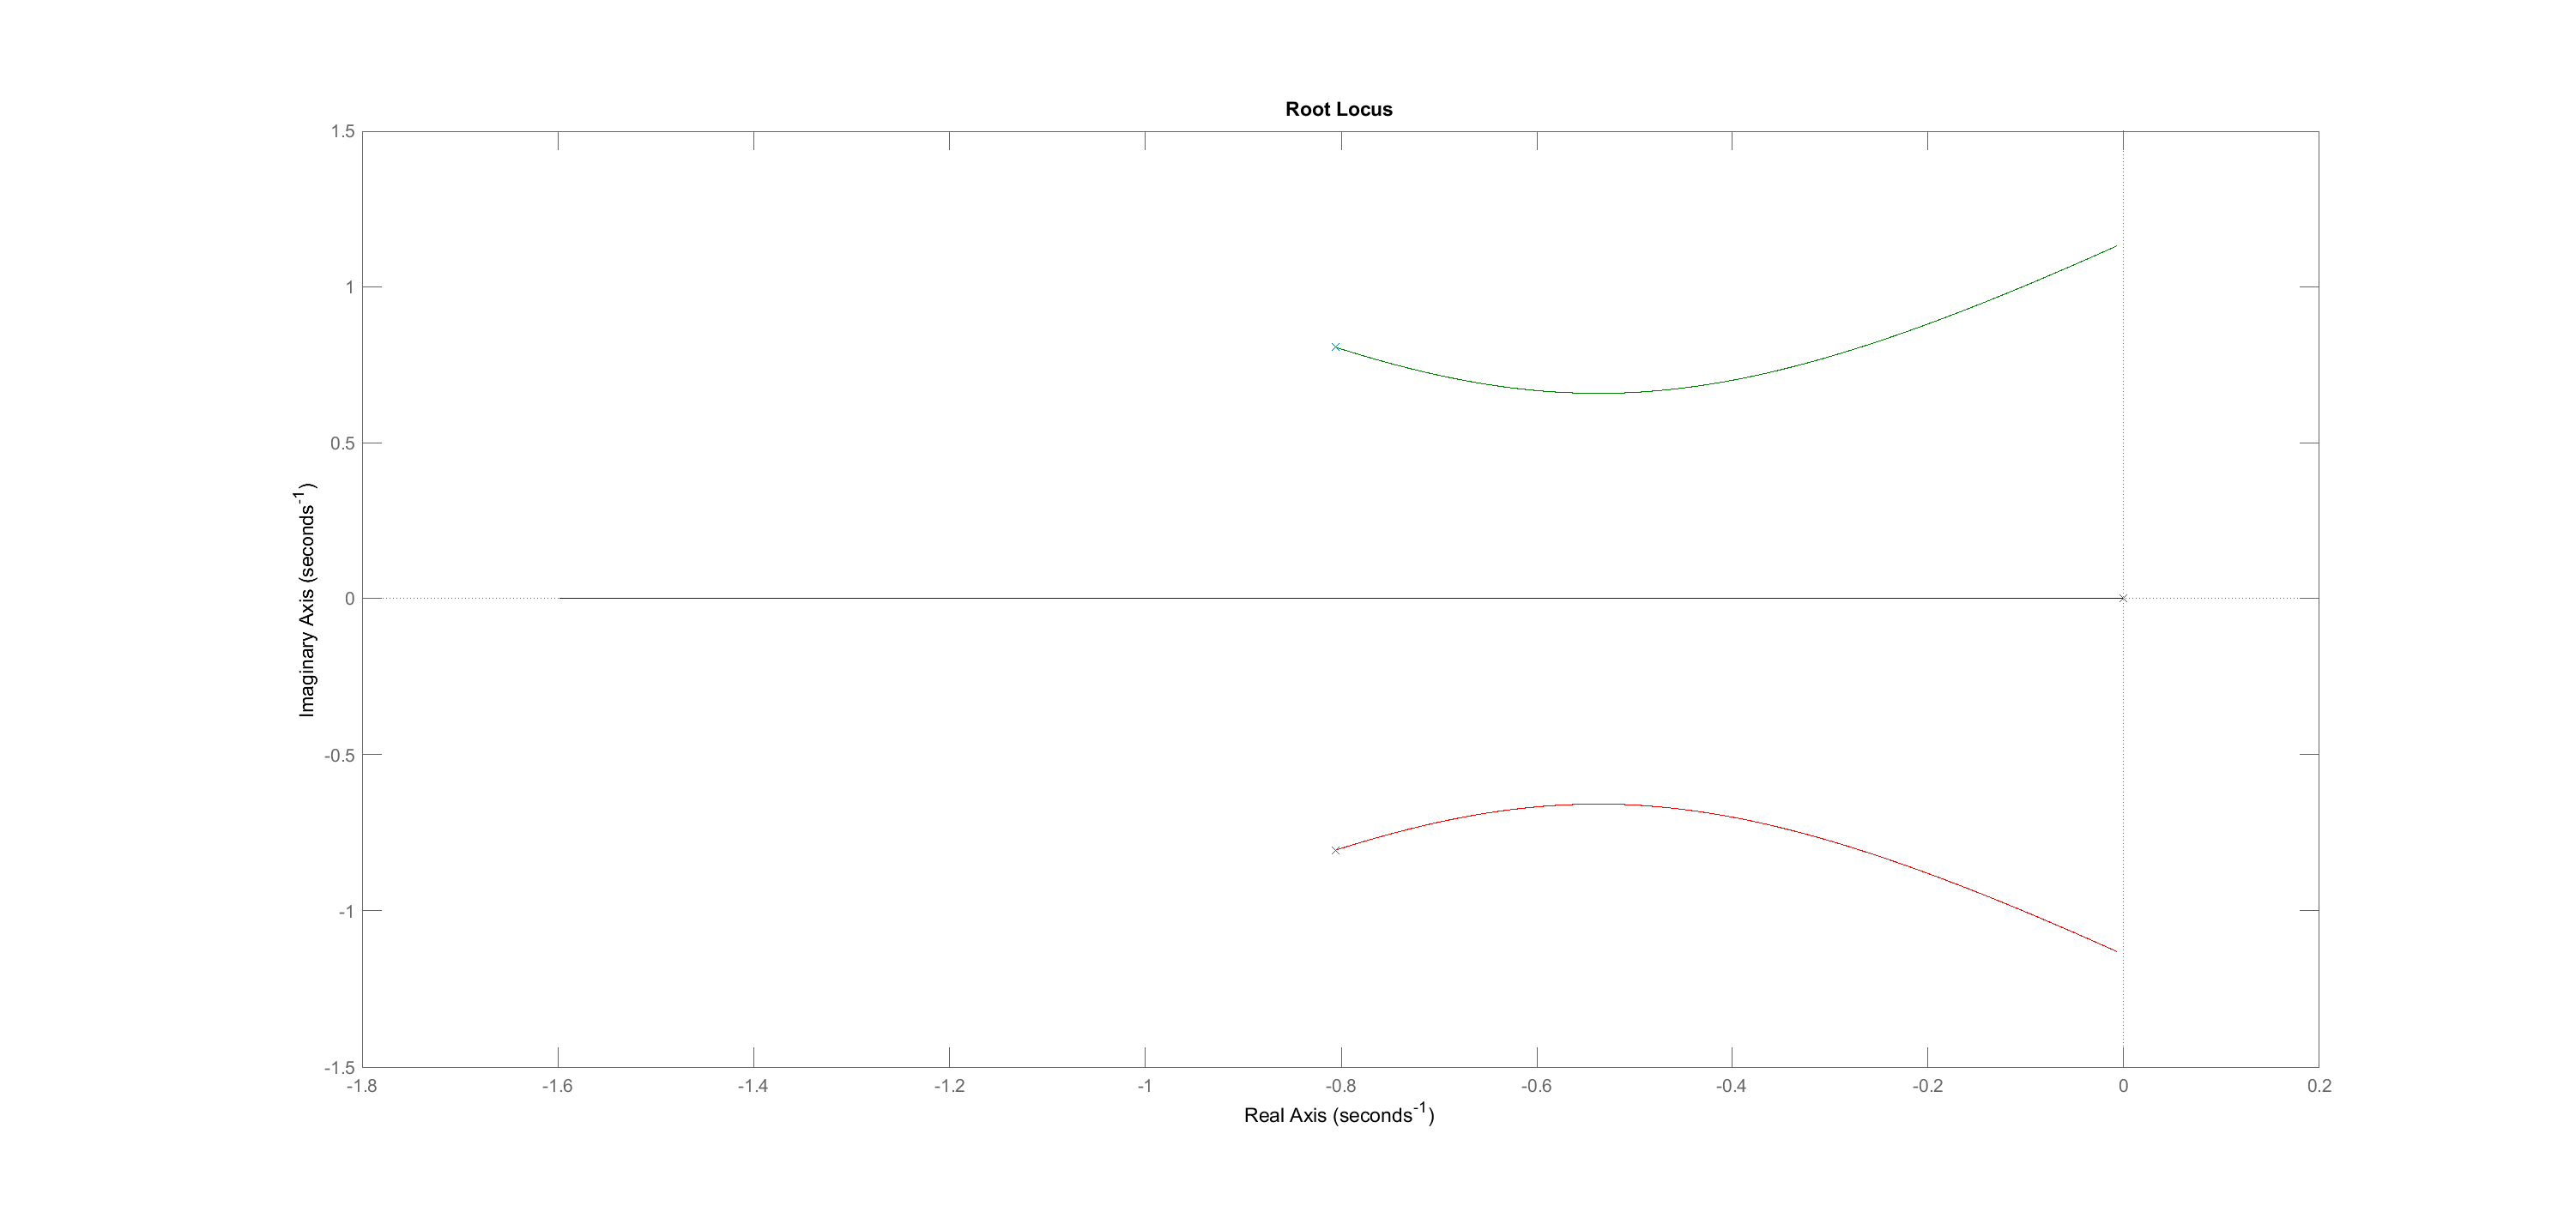
\includegraphics[width=\textwidth]{figures/root_locus_k_i_phi_interval_minus_pi_to_0}
		\caption{Root locus with range $k_{i_\phi}$ from -$\pi$ to 0}
		\label{fig:root_locus_proper_range}
	\end{subfigure}
\end{figure}

From this figure, we can conclude that the range seems to be slightly smaller than $-\pi$, but not by much, so that the range seems to be around $[-3.2, 0]$, but we are using $-\pi$ as it's a more interesting number. 

Further, choosing a lower $\omega_{n_\chi}$ by using $W_\chi = 10$ we may set $\zeta_\chi = 2$ a little higher without issue. Then we can find:
\begin{align*}
    \omega_{n_\chi} &= \frac{1}{W_\chi} \omega_{n_\phi} 
    = \frac{1}{10} 1.140 \approx 0.114 \\
    k_{p_\chi} &= \frac{2 \zeta_\chi \omega_{n_\chi} V_g}{g} 
    = \frac{2 * 2 * 0.114 * 580}{9.81 * 3.6} 
    \approx 7.49 \\
    k_{i_\chi} &= \frac{\omega_{n_\chi}^2 V_g}{g}
    = \frac{0.114^2 * 580}{9.81 * 3.6} 
    \approx 0.214
\end{align*}

\subsection{}
There doesn't seem like there's a need for an integrator for this model. The integrator is usually needed for removing a disturbance that enters before $\delta_a$ in Figure 1 of the assignment task. As there is no disturbance here, the only reason we'd need an integral term would be to stabilize the system, but we can see from the root-locus analysis that the system is stable for $k_{i_\phi} = 0$. Therefore, we may choose this value. 

\subsection{}
See the figures: 

\begin{figure}[ht]
	\centering
	\begin{subfigure}[b]{0.45\textwidth}
		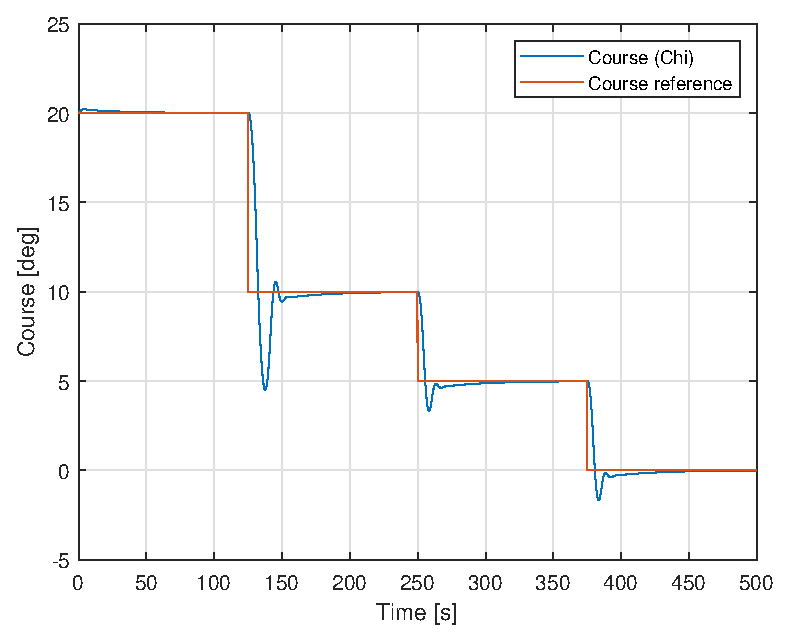
\includegraphics[width=\textwidth]{figures/2d_chi_course}
		\caption{The course and course reference $\chi$}
		\label{fig:2d_chi_course}
	\end{subfigure}
	\begin{subfigure}[b]{0.45\textwidth}
		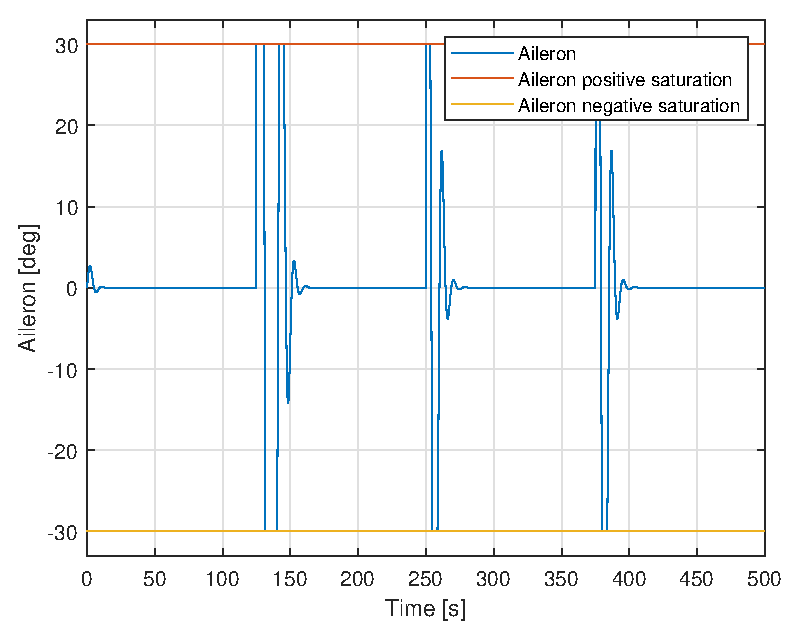
\includegraphics[width=\textwidth]{figures/2d_delta_a_aileron}
		\caption{The aileron with saturation $\delta_a$}
		\label{fig:2d_delta_a_aileron}
	\end{subfigure}
\end{figure}

The results seem decent in general, and we can note that the integral term for $\phi$ was unnecessary, as discussed earlier. 

\subsection{}
See the figures: 

\begin{figure}[ht]
	\centering
	\begin{subfigure}[b]{0.45\textwidth}
		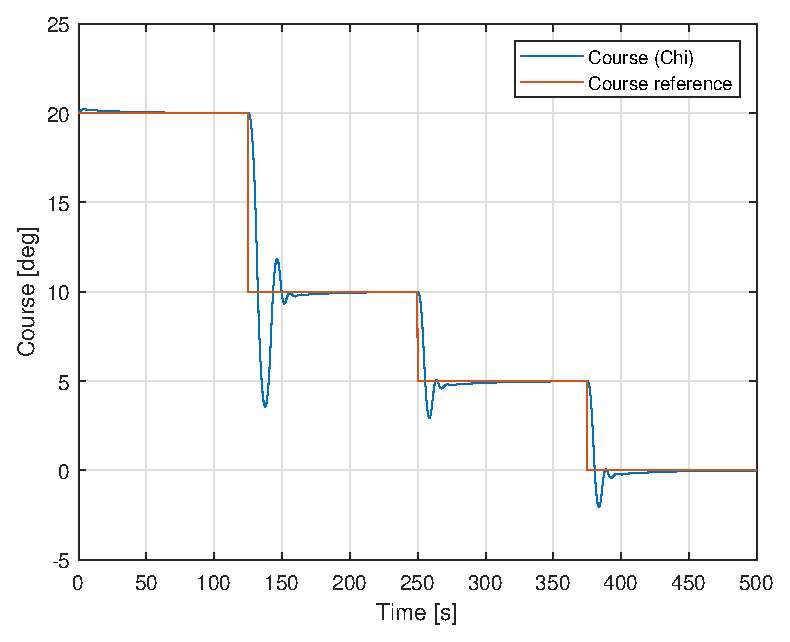
\includegraphics[width=\textwidth]{figures/2e_chi_course}
		\caption{The course and course reference $\chi$}
		\label{fig:2e_chi_course}
	\end{subfigure}
	\begin{subfigure}[b]{0.45\textwidth}
		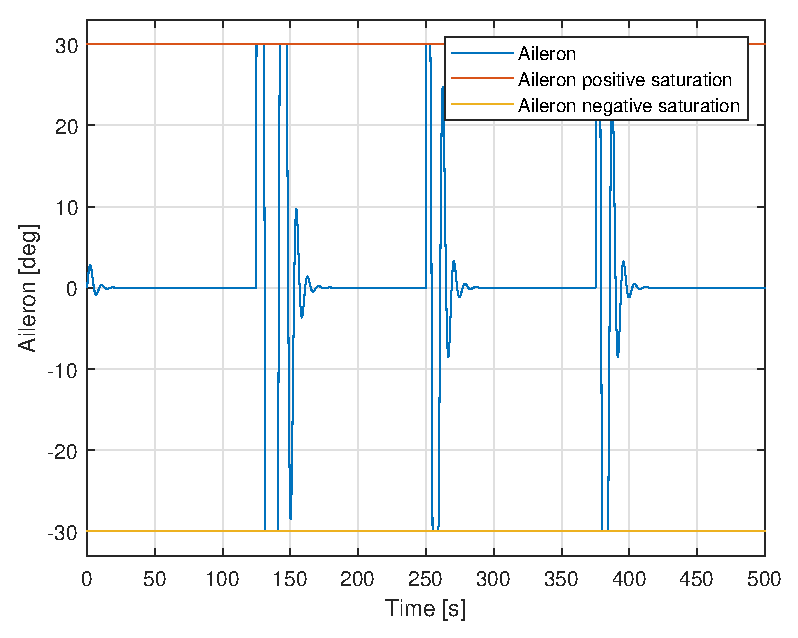
\includegraphics[width=\textwidth]{figures/2e_delta_a_aileron}
		\caption{The aileron with saturation $\delta_a$}
		\label{fig:2e_delta_a_aileron}
	\end{subfigure}
\end{figure}